% With a state of the art detector and three years worth of data, an analysis is in progress to look for di-Higgs processes. The production mode that will considered is gluon gluon fusion:

% \begin{figure}[H]%
%     \setcounter{subfigure}{0} % reset subcaption counter to 0 (a) 
%     \centering
%     \subfloat[SM Box Diagram]{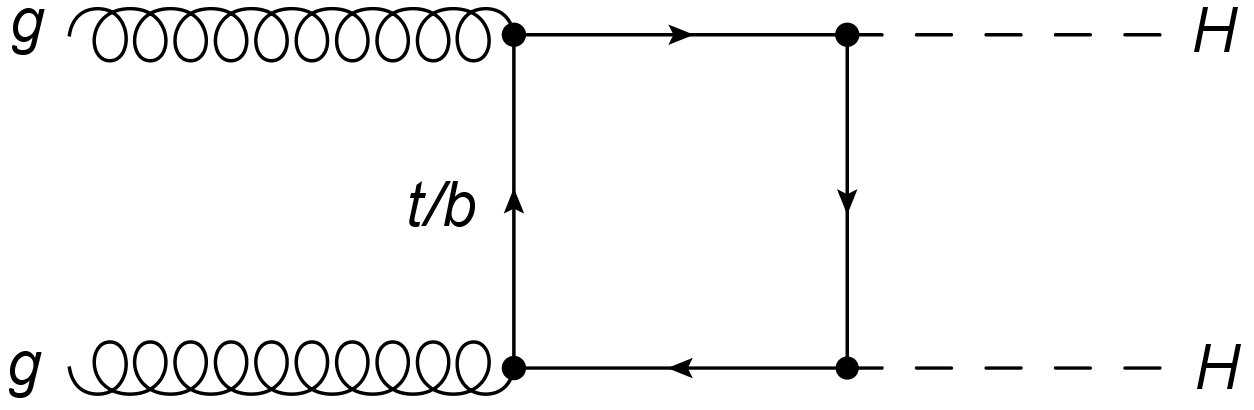
\includegraphics[width=.4\linewidth]{Images/FD_HH_Box.png}}%
%     \qquad
%     \subfloat[SM Triangle  Diagram]{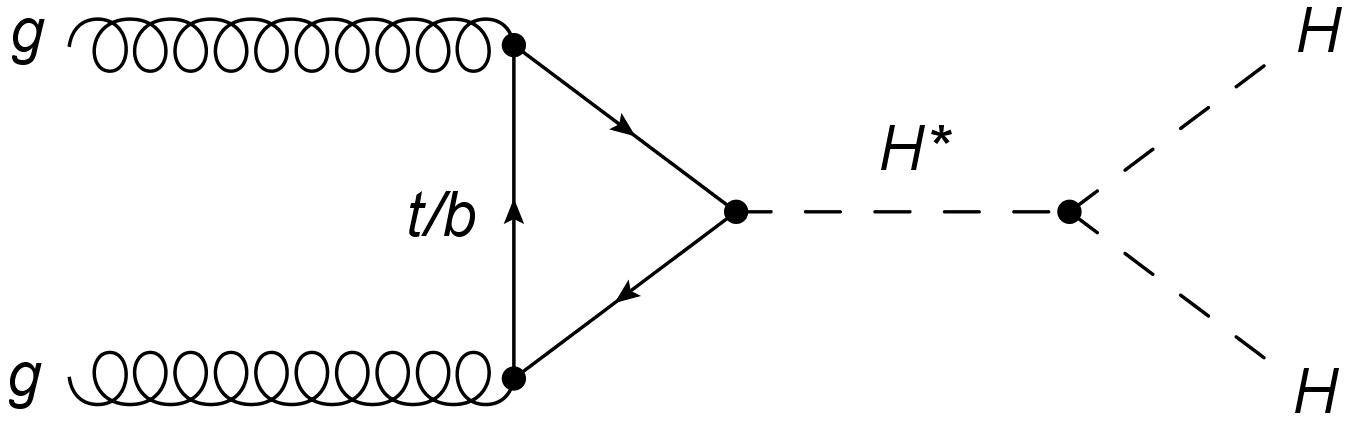
\includegraphics[width=.42\linewidth]{Images/FD_HH_Tri.png}}%
%     \caption{The leading order Feynman diagrams for gluon-gluon fusion di-Higgs production.}%
% \end{figure}

% In this process, two gluons with a large fraction of their protons' momentum interact and create two Higgs bosons via a heavy quark loop. The two major leading order diagrams are the `box' and `triangle' diagrams. In the SM, these diagrams destructively interfere, leading to a production cross section on order 1000 times less than that of single Higgs boson production, about 50 pb compared to about 30 fb \cite{sigma_ggH} \cite{sigma_ggHH}. The di-Higgs process can also be produced through a BSM resonant particle, as in the following diagram:

% \begin{figure}[H]
% \centering
% 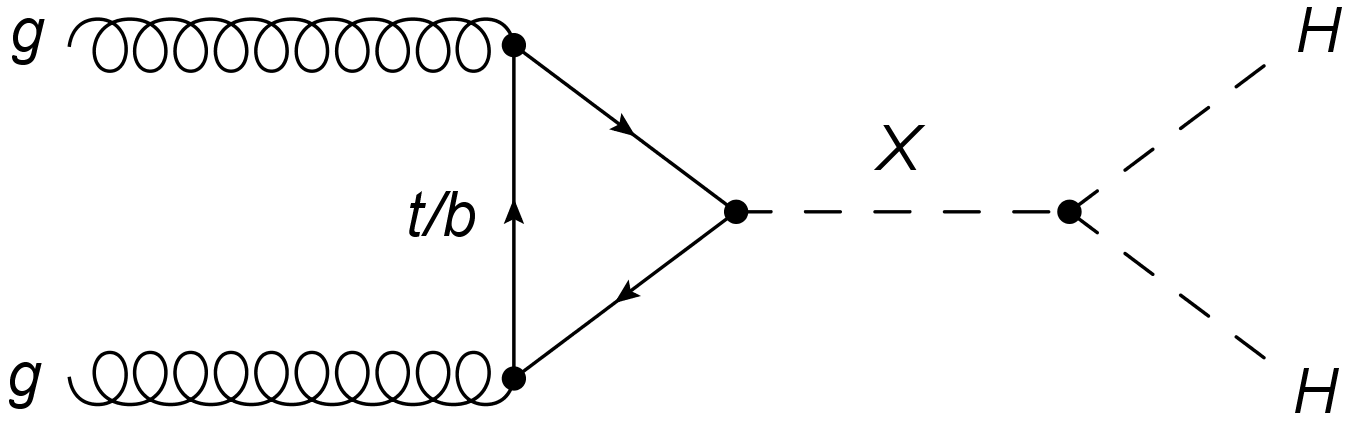
\includegraphics[width=.42\linewidth]{Images/FD_XHH.png}
% \caption{BSM Heavy Resonance Diagram}
% %\label{fig:7}
% \end{figure}

% where `X' is a heavy resonant particle, which may be a radion or graviton, that decays into two Higgs bosons \cite{radion_kkgraviton}. When this third diagram is added, the cross section of di-Higgs production is increased. 

% \subsection{Introduction}

% The Higgs decay modes that will be considered for this analysis is HH$\rightarrow WW\gamma\gamma$. In this decay channel, one Higgs boson decays into two W bosons, and the other decays into two photons. While this process has a low branching ratio of $\approx$ 0.1\%, one can use the very high $H\rightarrow\gamma\gamma$ mass precision to improve the signal to background ratio. 

% \begin{figure}[H]
% \centering
% 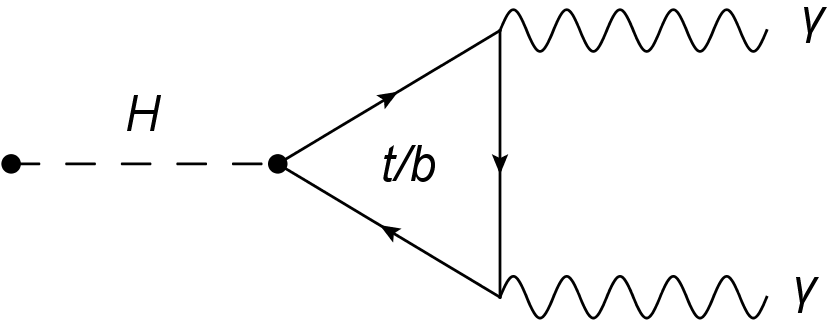
\includegraphics[width=.3\linewidth]{Images/H_gg.png}
% \caption{Higgs to two photons Feynman diagram}
% %\label{fig:7}
% \end{figure}

% \begin{figure}[H]%
%     \setcounter{subfigure}{0} % reset subcaption counter to 0 (a) 
%     \centering
%     \subfloat[Semi-leptonic H$\rightarrow WW$ decay]{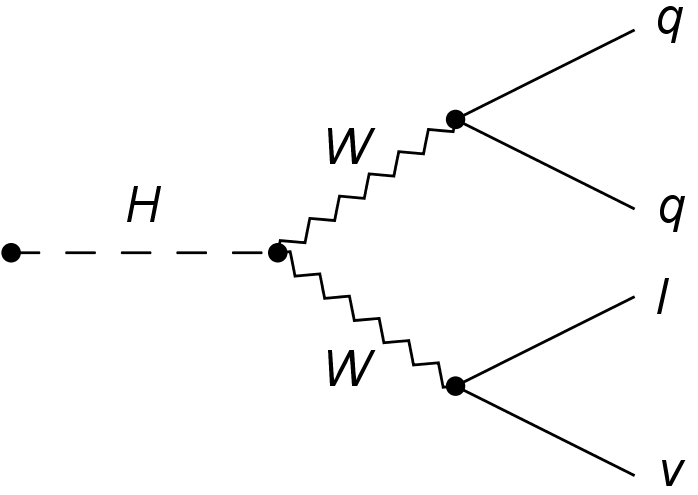
\includegraphics[width=.3\linewidth]{Images/FD_HH_qqlnu.png}}%
%     \qquad
%     \subfloat[Fully-leptonic H$\rightarrow WW$ decay]{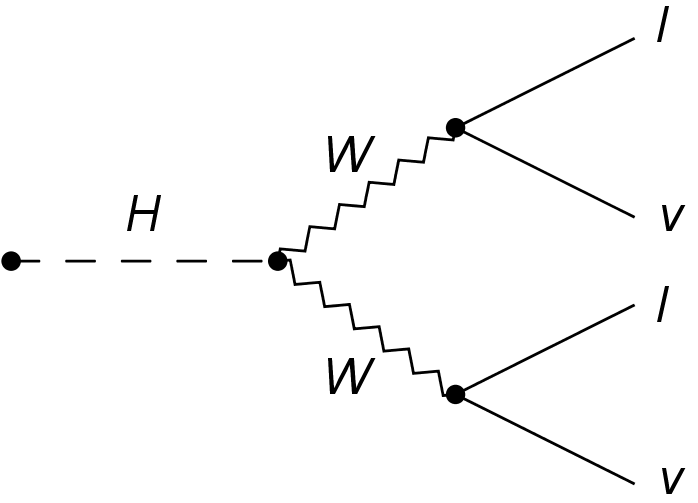
\includegraphics[width=.3\linewidth]{Images/FD_HH_lnulnu.png}}%
%     \qquad
%     \subfloat[Fully-hadronic H$\rightarrow WW$ decay]{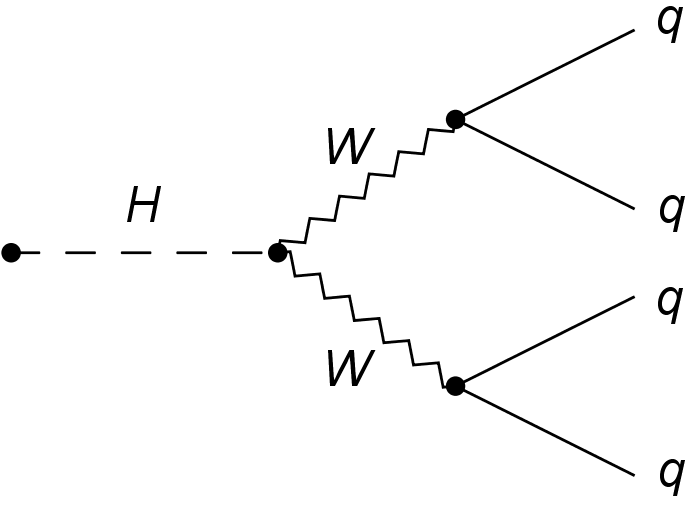
\includegraphics[width=.3\linewidth]{Images/FD_HH_qqqq.png}}%
%     \caption{Feynman diagrams for the three decay modes of $H\rightarrow WW$.}%
% \end{figure}

% This channel has been searched for by ATLAS, the other general-purpose detector at the LHC, with 8 TeV \cite{atlas1} and 13 TeV data \cite{atlas2}. At the conclusion of this analysis, a result comparison can be made. In addition, the result of the analysis can be combined with the other HH decay channels studied by the CMS HH group for a more precise result.  

% \subsection{Strategy}

% Two measurements that can be performed under an SM di-Higgs analysis is that of the self-Higgs coupling, and the production cross-section of a non-resonantly produced pair of Higgs bosons. It is  not expected that the Run 2 dataset (2016-2018) will be large enough to perform these measurements, as the cross section for SM di-Higgs is extremely small, as described earlier. However, BSM processes may enhance the di-Higgs cross section.

% Because of this, expected results of the analysis include a computation of the upper limit of non-resonant HH production and resonant HH production from a BSM particle. The BSM production limit can be computed for different heavy resonance masses, corresponding to different assumptions of the BSM particle's mass. The current plan is to perform the analysis in the non-boosted regime of 250 GeV to 1000 GeV, and depending on the result from this analysis, the boosted regime mass range of 1 TeV to 3 TeV may also be studied. Higher mass points are in the boosted regime because the Higgses, which result from the decay of the heavy BSM particle, would be produced with high momentum, leading to a potentially different analysis strategy.

% As in most analyses, selections will be made on the events recorded by CMS. This means that events will not be selected if they don't match the criteria of expected events from the signal. When defining the selection, an optimization will be made between maintaining a high signal efficieny for HH$\rightarrow WW\gamma\gamma$ events, while rejecting as much background as possible.

% An example of a signal region, the one used by the CMS $H\rightarrow\gamma\gamma$ analysis, is the di-photon mass near 125 GeV. This is used as a signal region because if the passed events are truly from the expected signal, the invariant mass of the two photons should be close to that of the SM Higgs boson.

% \subsection{Results}

% The selections, categorization, and analytic fitting methods previously described can be applied to CMS data and different simulated signal samples. Different simulated signal samples and an EFT approach are used to constrain various EFT parameters in an HH scenario, and upper limits are observed for varying benchmark BSM scenarios.  

% \subsubsection{Standard Model}

% %%-- Standard model diagram 
% \begin{figure}[H]
%     \centering
%     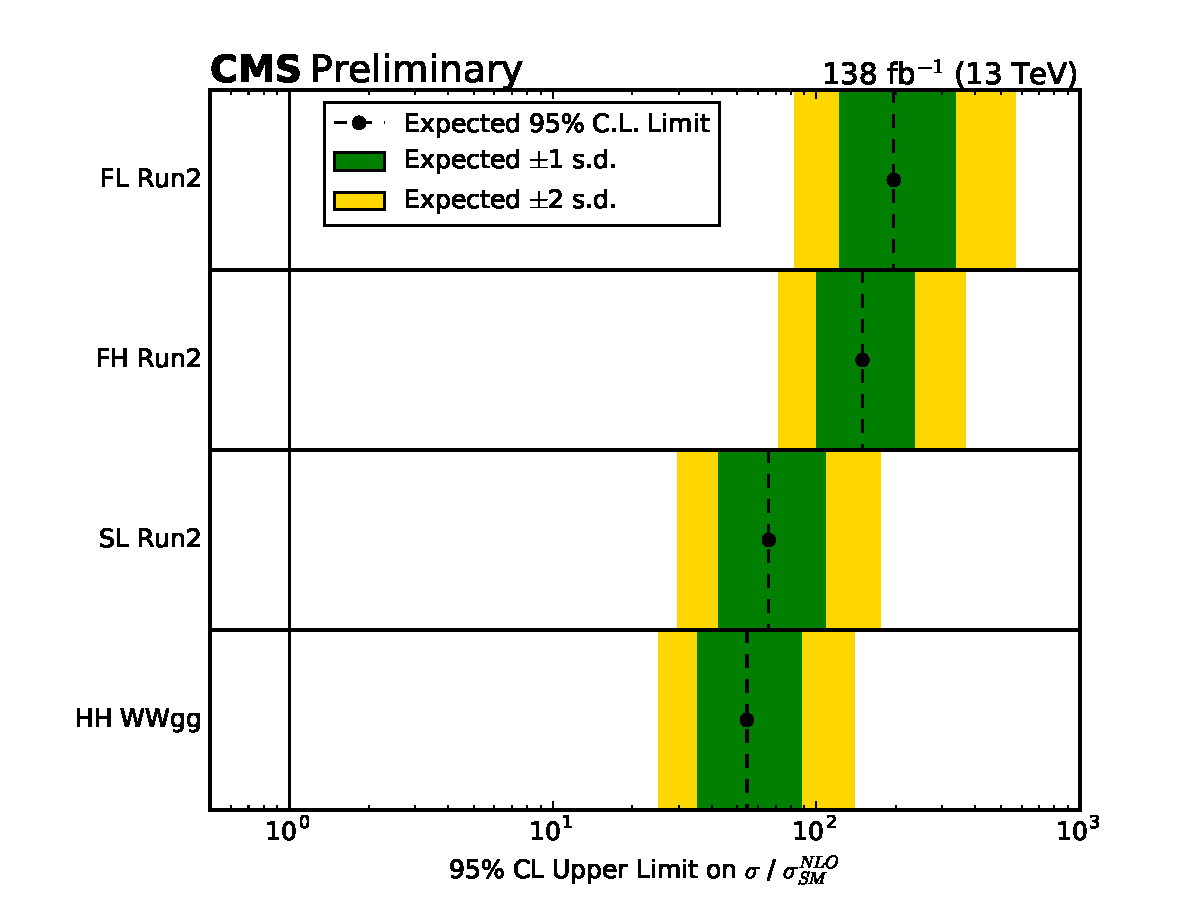
\includegraphics[width=0.65\textwidth]{Images/Results/SM_UpperLimits.pdf}
%     \caption{95\% CL limits on HH gluon gluon fusion production with respect to $\sigma^{SM}_{NLO}$ = 31.05 fb}
%     \label{fig:SM_Result}
% \end{figure}

% \subsubsection{Higgs self-coupling scan}

% \subsubsection{di-Higgs to two gluon coupling scan}

% \subsubsection{EFT benchmarks}

% \subsection{Summary}

% \subsection{Extra}

% Because the main decay modes of the W boson include both a di-quark and lepton-neutrino decay, a di-Higgs decay into two W bosons can have three types of final states: semi-lptonic (SL), fully-leptonic (FL) and fully-hadronic (FH). These correspond to the three W boson decay combinations, yielding final states of qql$\nu$, l$\nu$l$\nu$ and qqqq respectively. In order to have an idea of signal efficiency and an understanding of the signal process, private samples have been produced for the three decay channels. These samples were produced with MadGraph5$\_$aMC$@$NLO and Pythia 8. 

% A simulated signal sample is our most accurate model of the distributions of experimental observables. The first step of a signal process simulation, the GEN (generation) step, contains in its output physical variables of the particles involved in the process. This includes the transverse momentum $p_{T}$ with respect to the beam axis of the Higgs bosons. 

% After the GEN step, the interaction of the outgoing particles with the CMS detector is simulated, allowing one to reconstruct particle observables. This can be done for the diphoton object created post detector-simulation, a pair of photon objects which are presumed to have come from one of the Higgs bosons in the original process:

% \begin{figure}[H]%
%     \setcounter{subfigure}{0} % reset subcaption counter to 0 (a) 
%     \centering
%     \subfloat[Semi-leptonic]{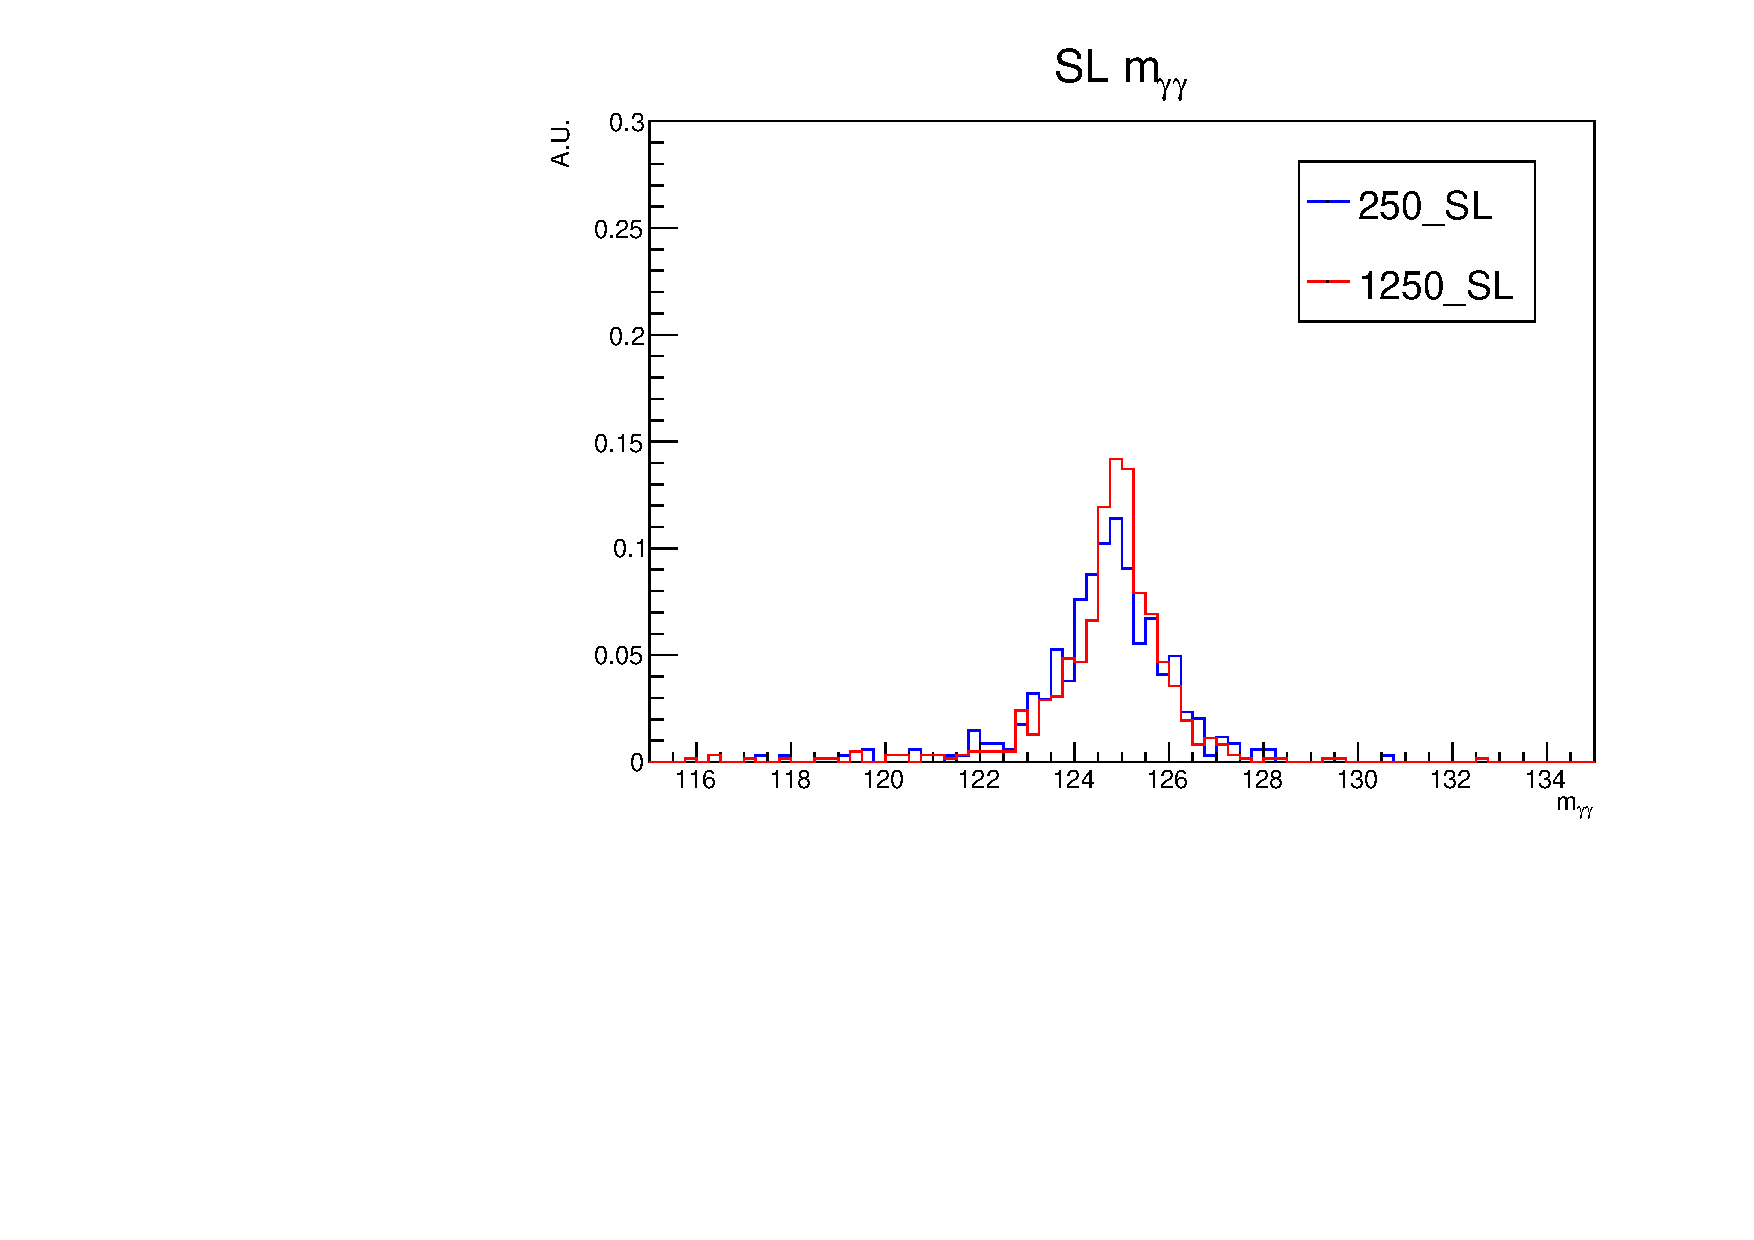
\includegraphics[width=.3\linewidth]{Images/SL_mgg.pdf}}%
%     \qquad
%     \subfloat[Fully-leptonic]{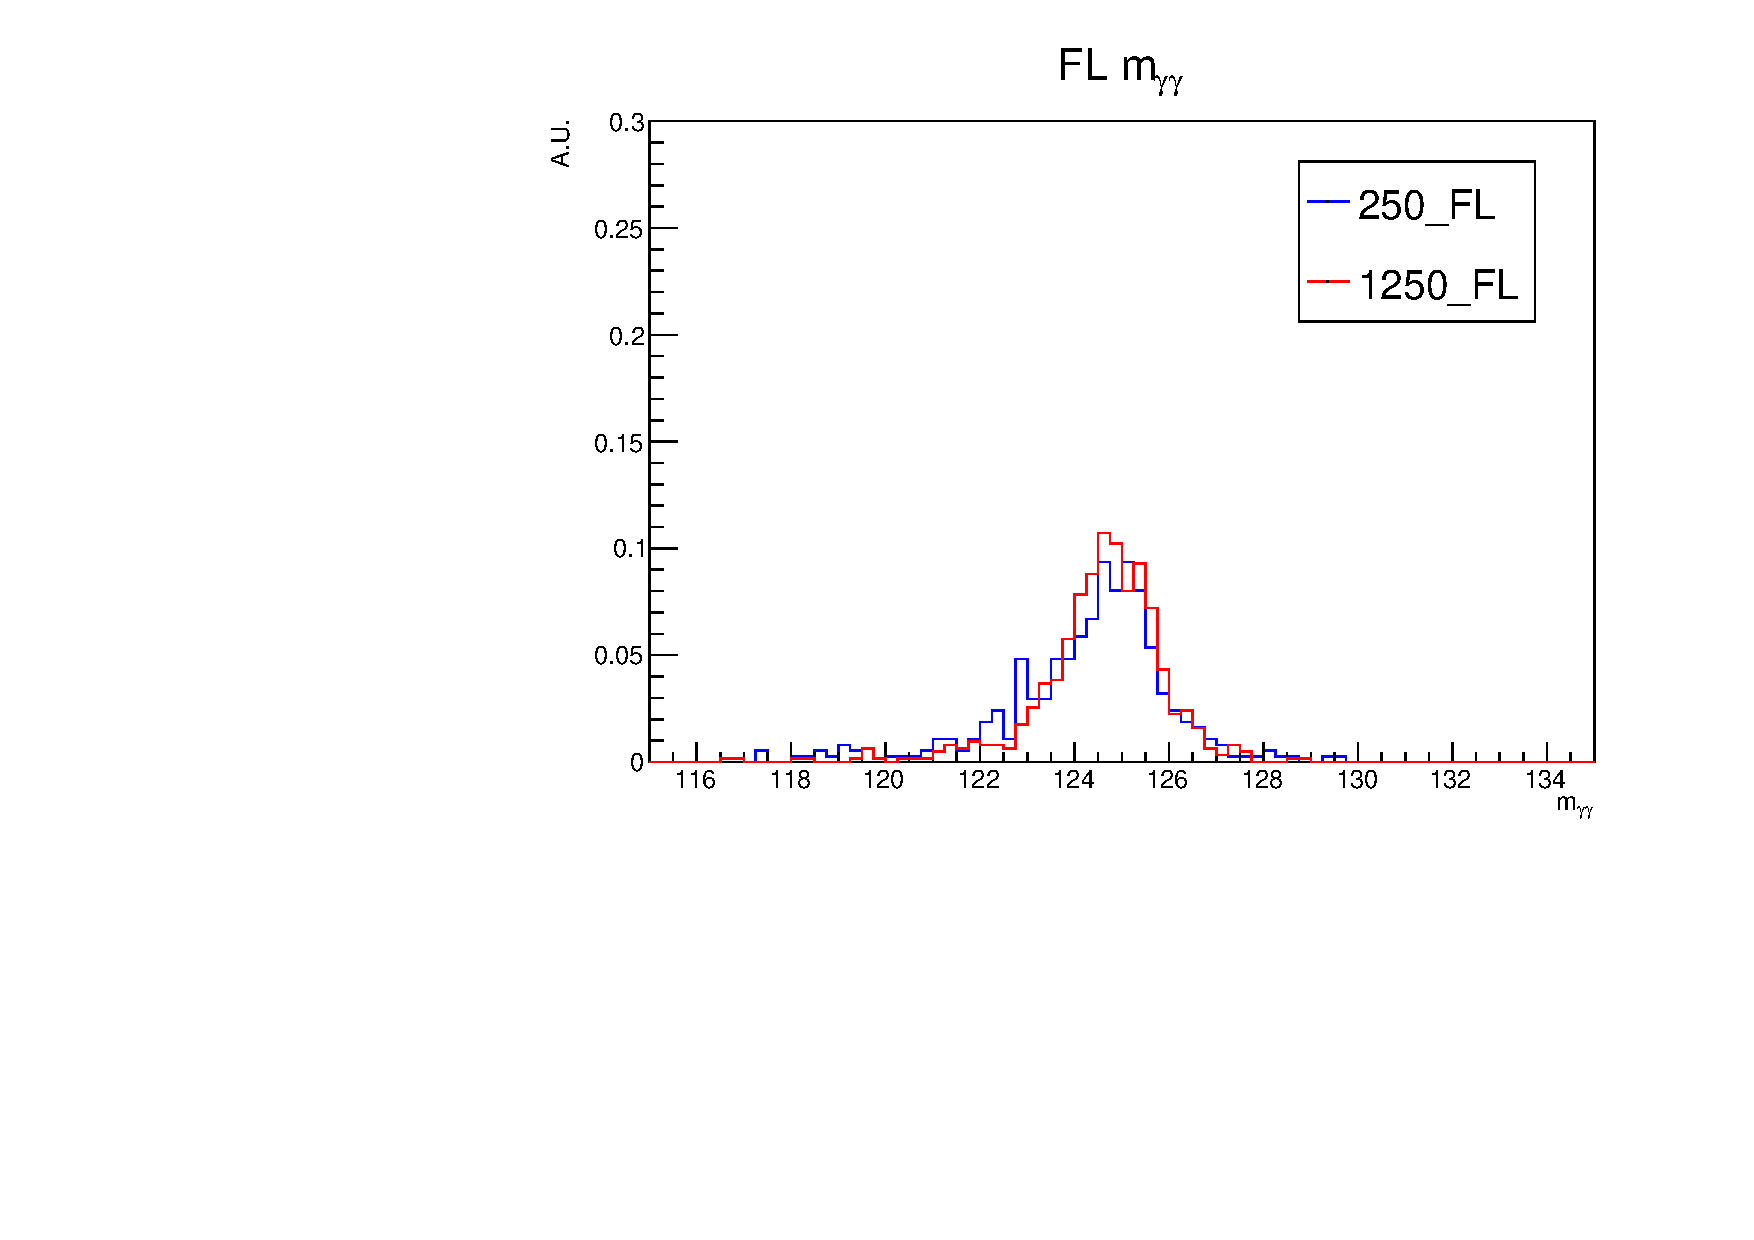
\includegraphics[width=.3\linewidth]{Images/FL_mgg.pdf}}%
%     \qquad
%     \subfloat[Fully-hadronic]{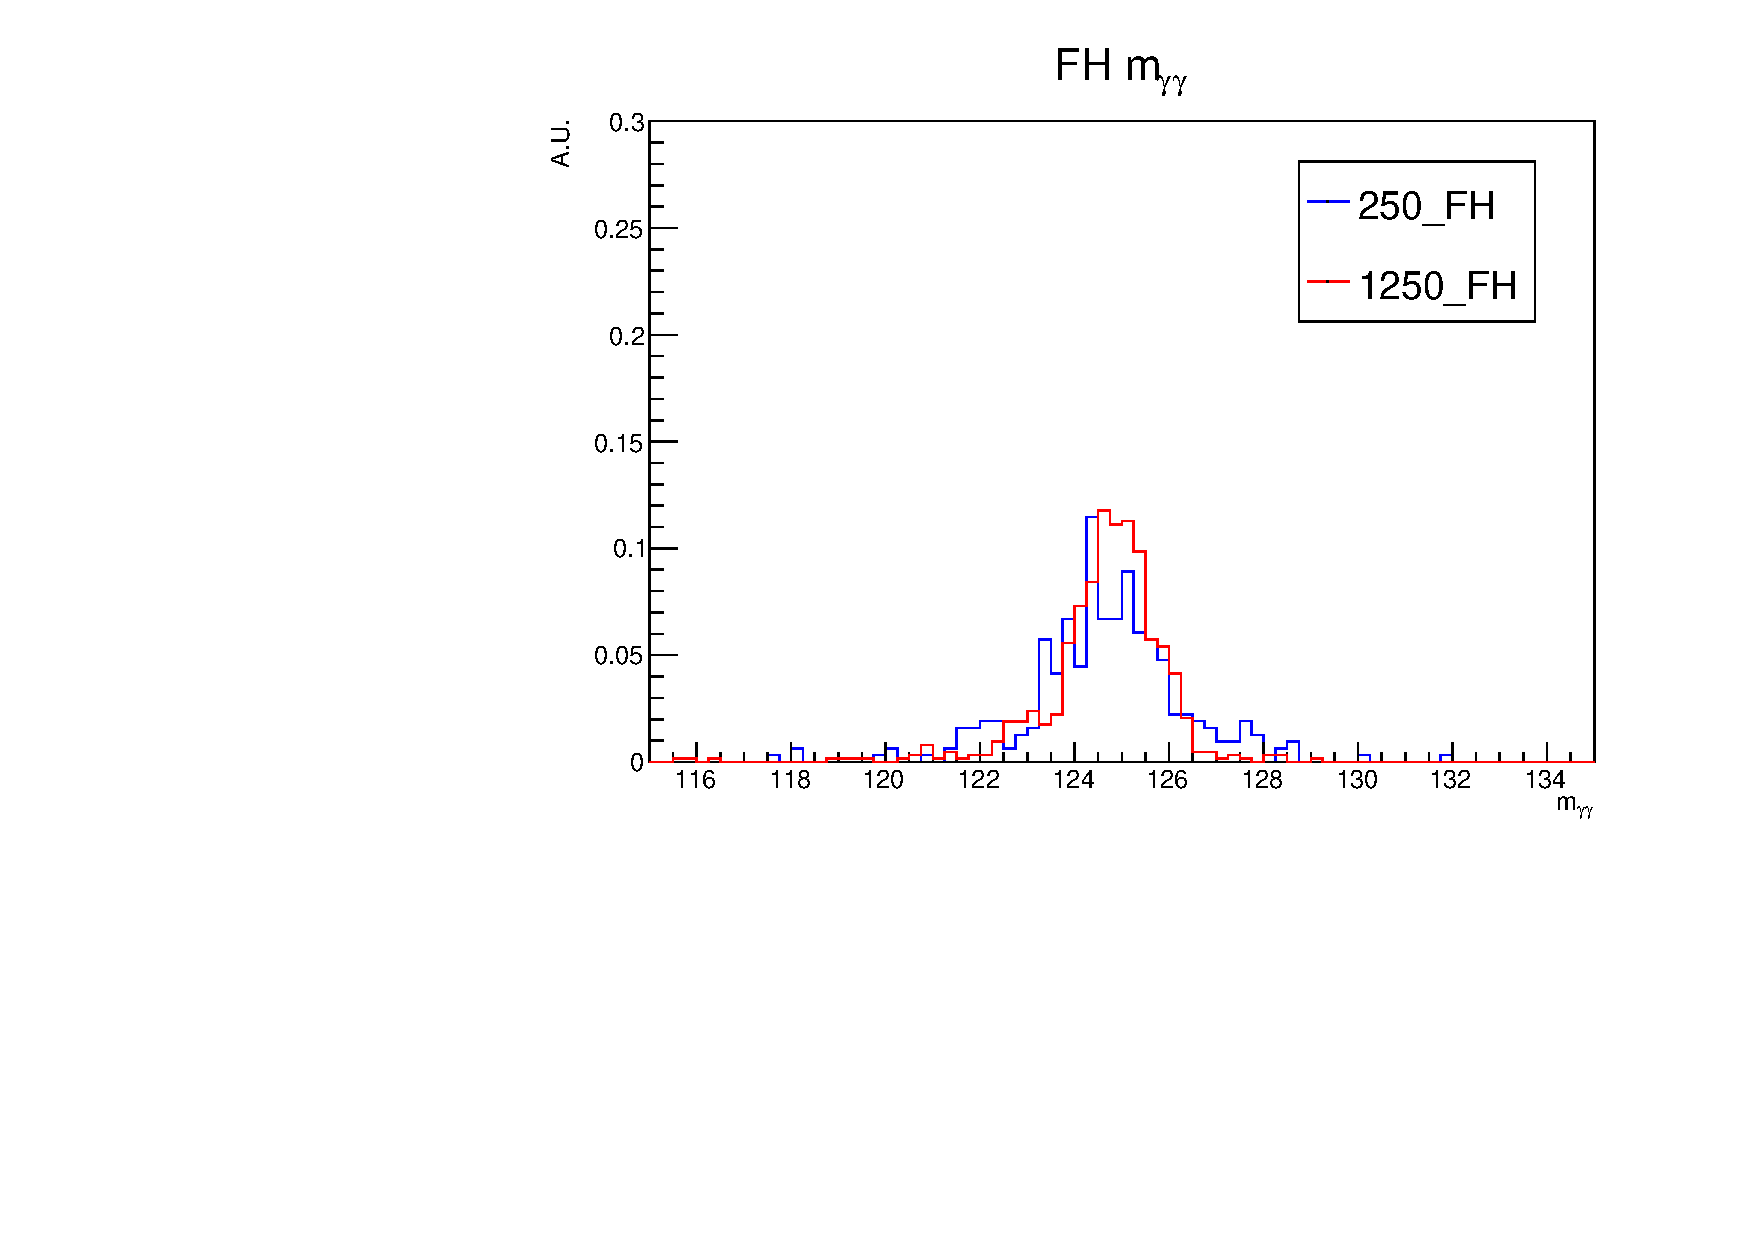
\includegraphics[width=.3\linewidth]{Images/FH_mgg.pdf}}%
%     \caption{Invariant mass of the leading diphoton object in the three WW decay modes for mass points 250 GeV and 1250 GeV. For each distribution, the integral is normalized to one.}%
% \end{figure}

% \begin{figure}[H]%
%     \setcounter{subfigure}{0} % reset subcaption counter to 0 (a) 
%     \centering
%     \subfloat[Semi-leptonic]{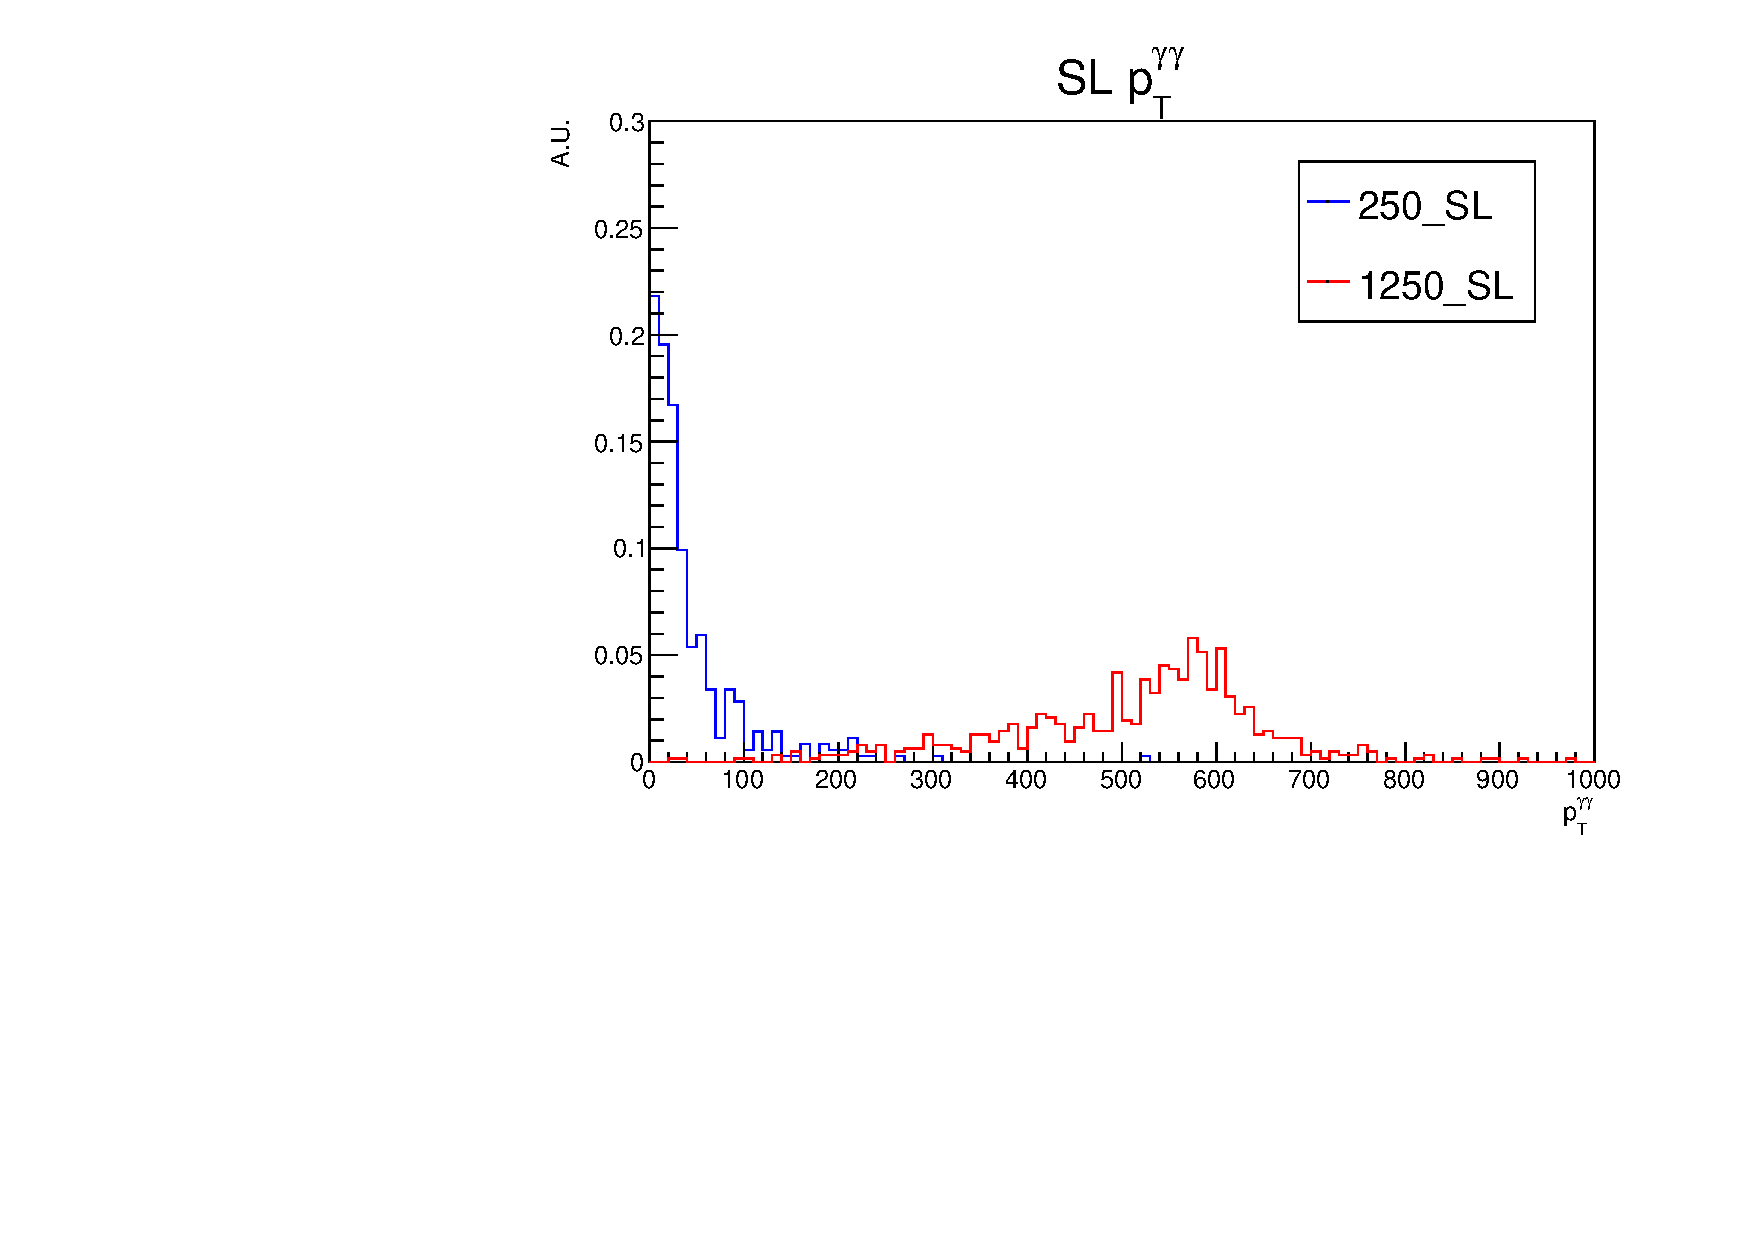
\includegraphics[width=.3\linewidth]{Images/SL_ptgg.pdf}}%
%     \qquad
%     \subfloat[Fully-leptonic]{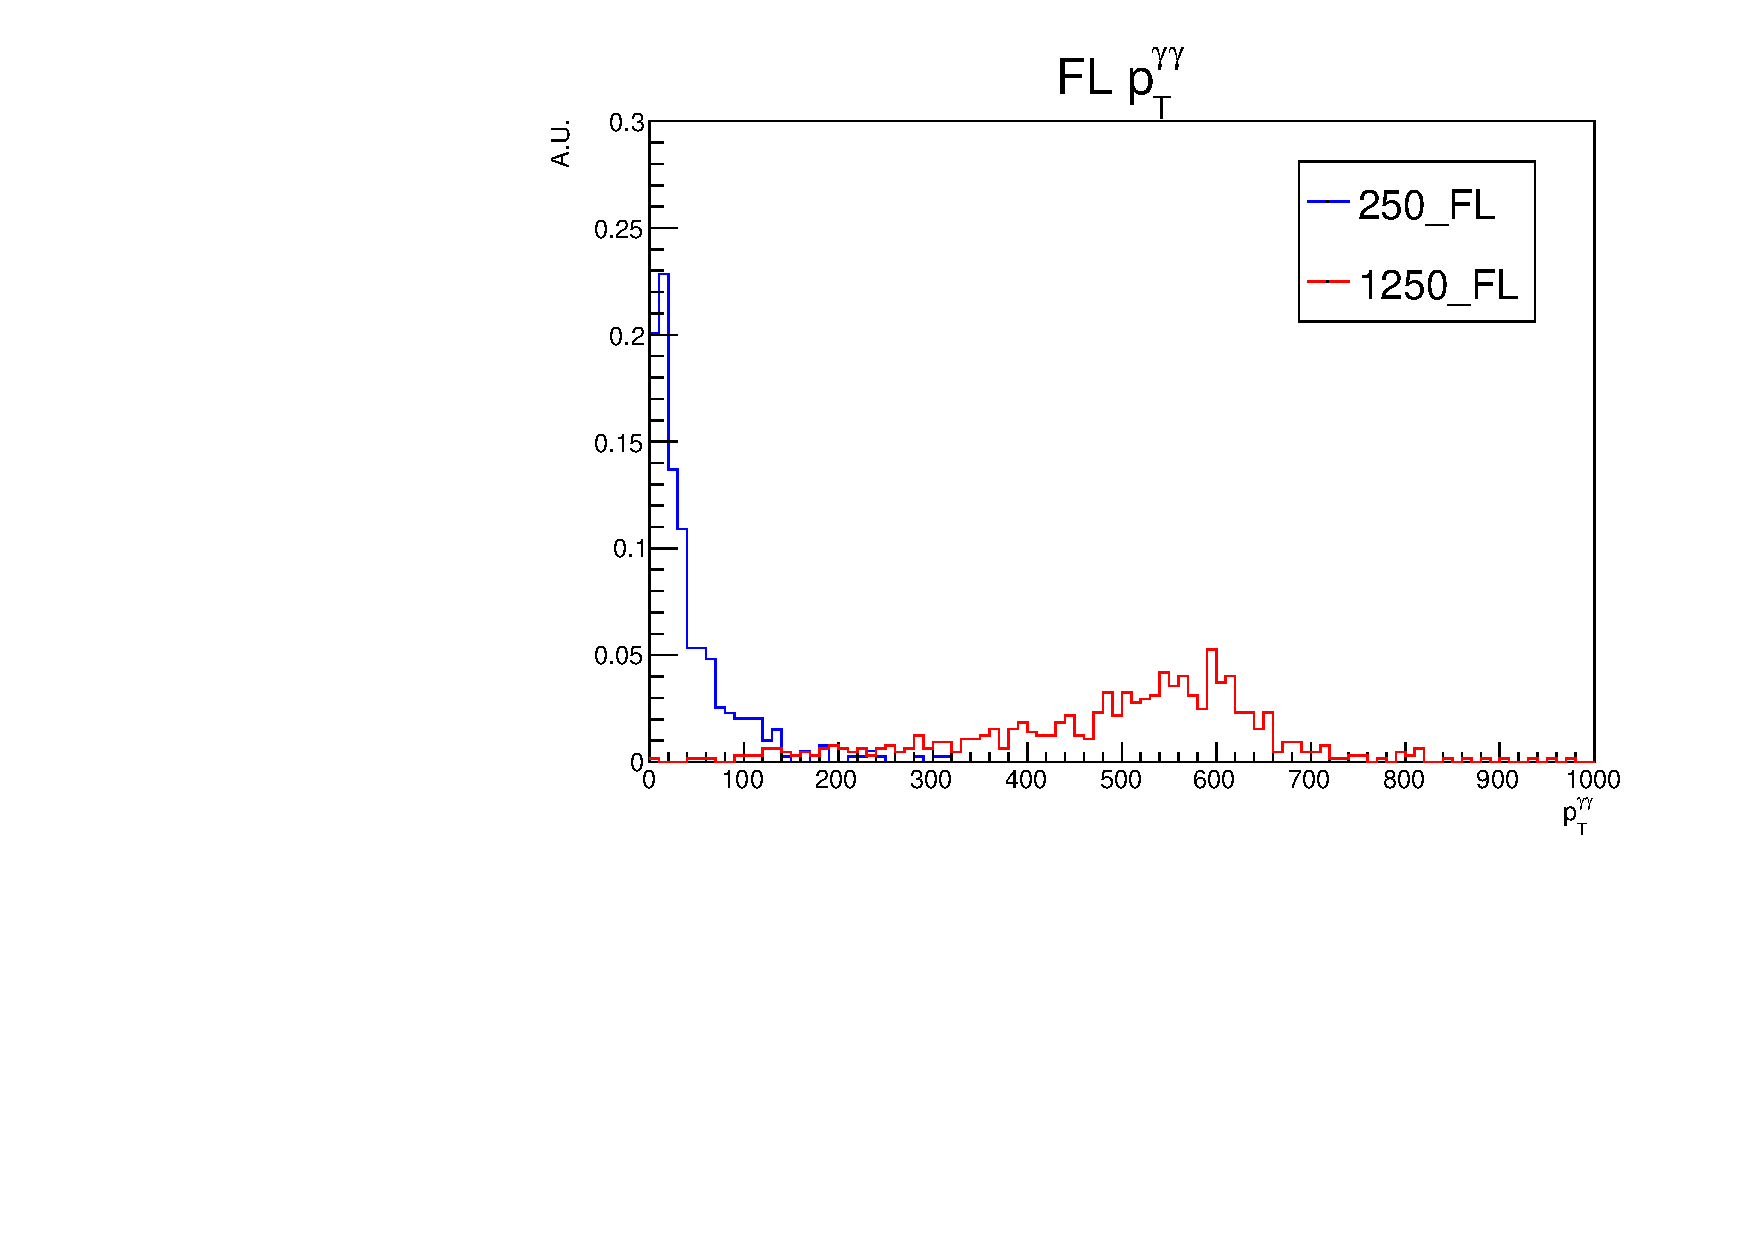
\includegraphics[width=.3\linewidth]{Images/FL_ptgg.pdf}}%
%     \qquad
%     \subfloat[Fully-hardonic]{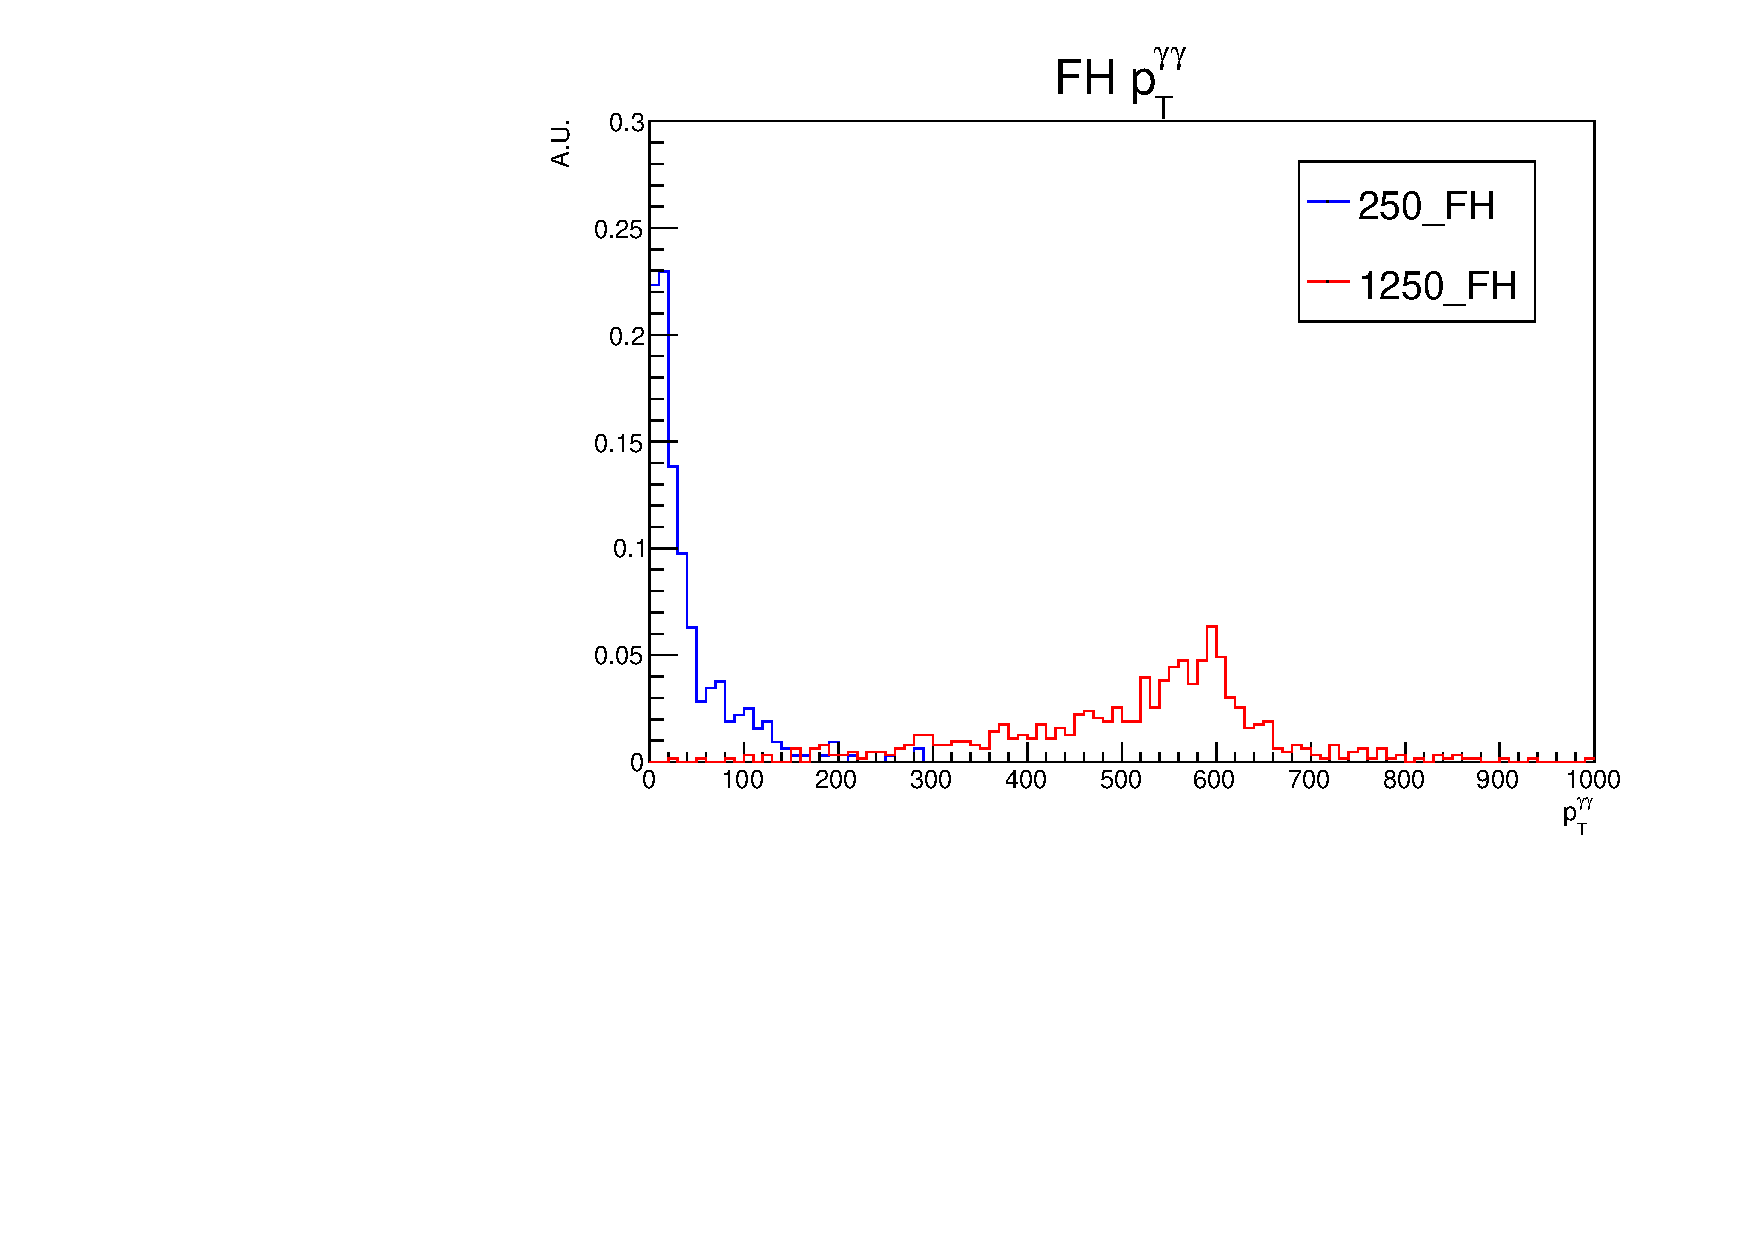
\includegraphics[width=.3\linewidth]{Images/FH_ptgg.pdf}}%
%     \caption{$p_{T}$ of the leading diphoton object for the three decay channels for mass points 250 GeV and 1250 GeV. For each distribution, the integral is normalized to one.}%
% \end{figure}

% \begin{figure}[H]
%     \centering
%     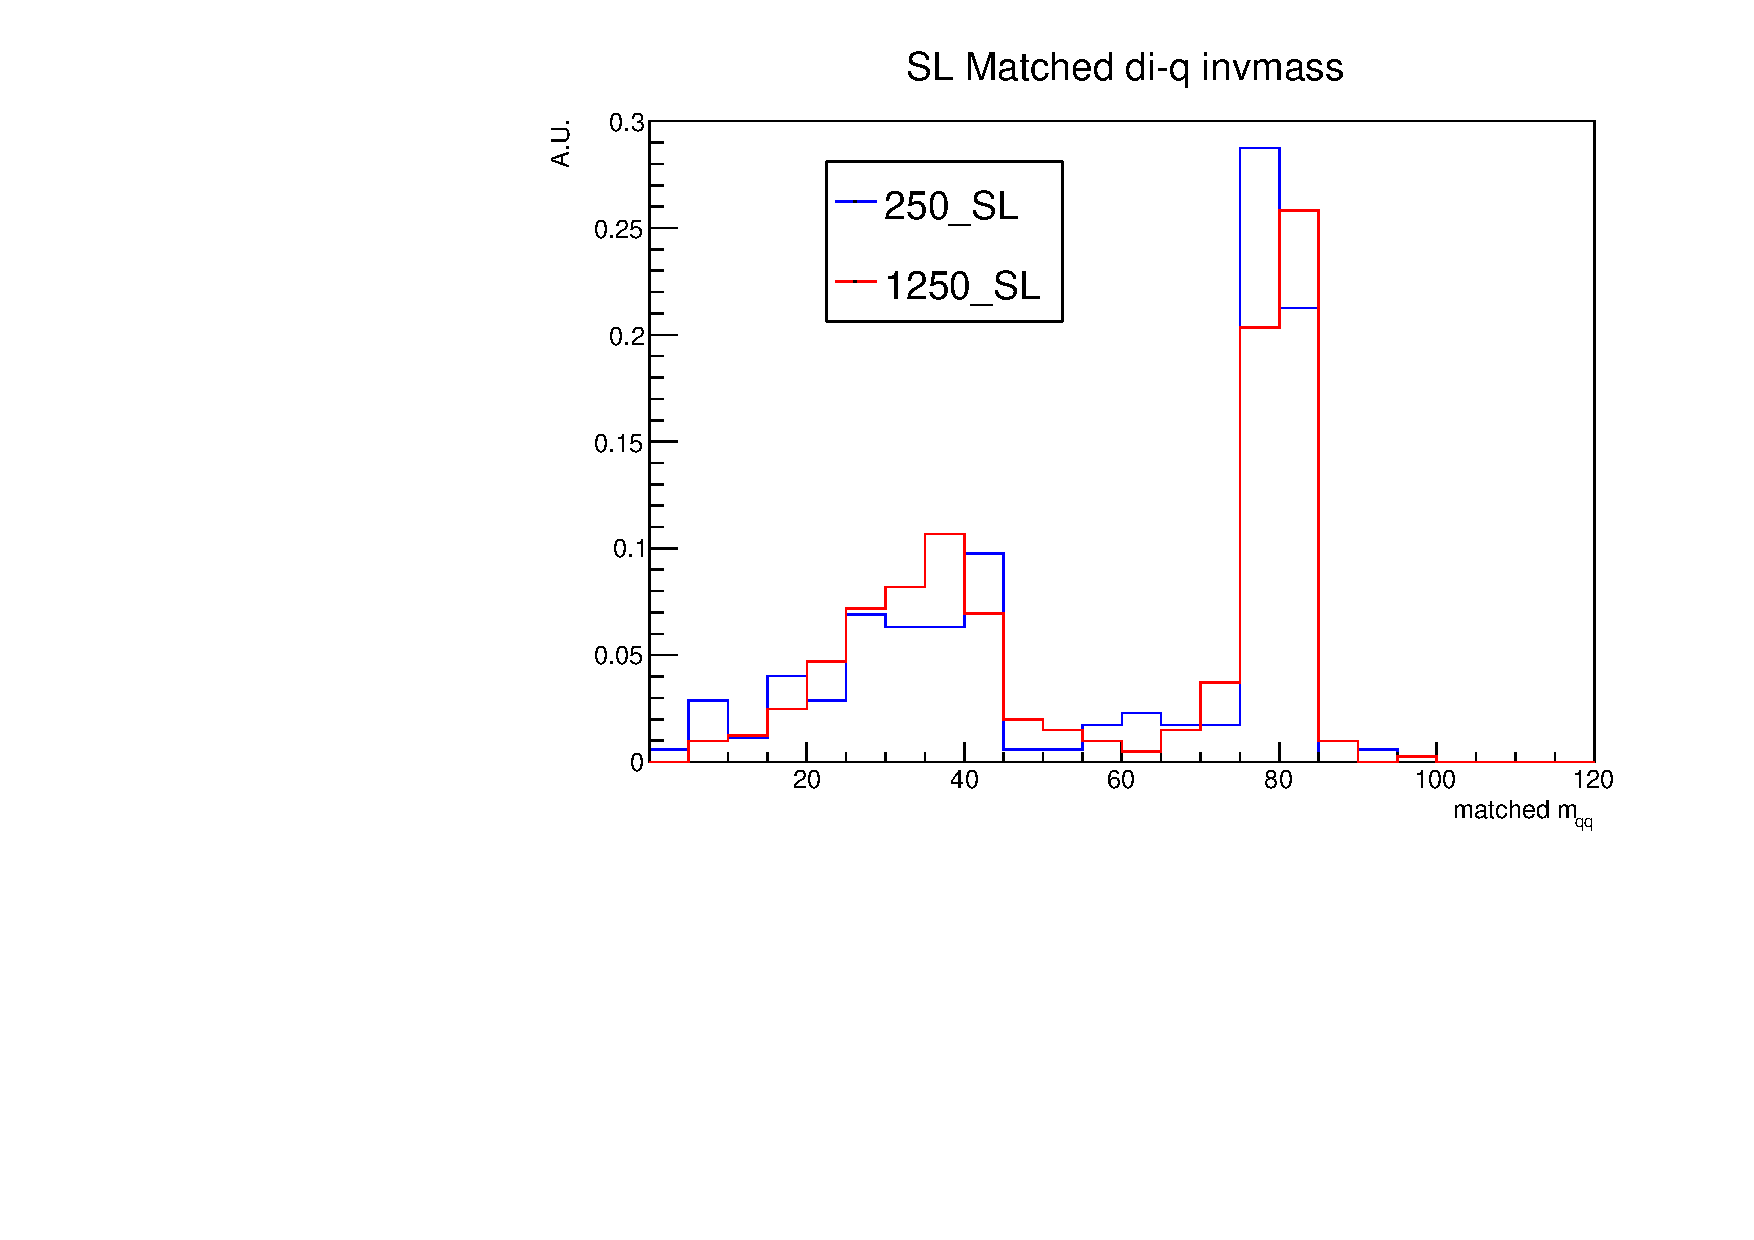
\includegraphics[width=.5\linewidth]{Images/SL_Matched_mqq.pdf}
%     \caption{Invariant mass of the two jets with the closest $\Delta R$ ($\sqrt{\Delta \phi ^{2} + \Delta \eta ^{2}}$) to the GEN quarks.}
% \end{figure}

% % \begin{figure}[H]
% %     \centering
% %     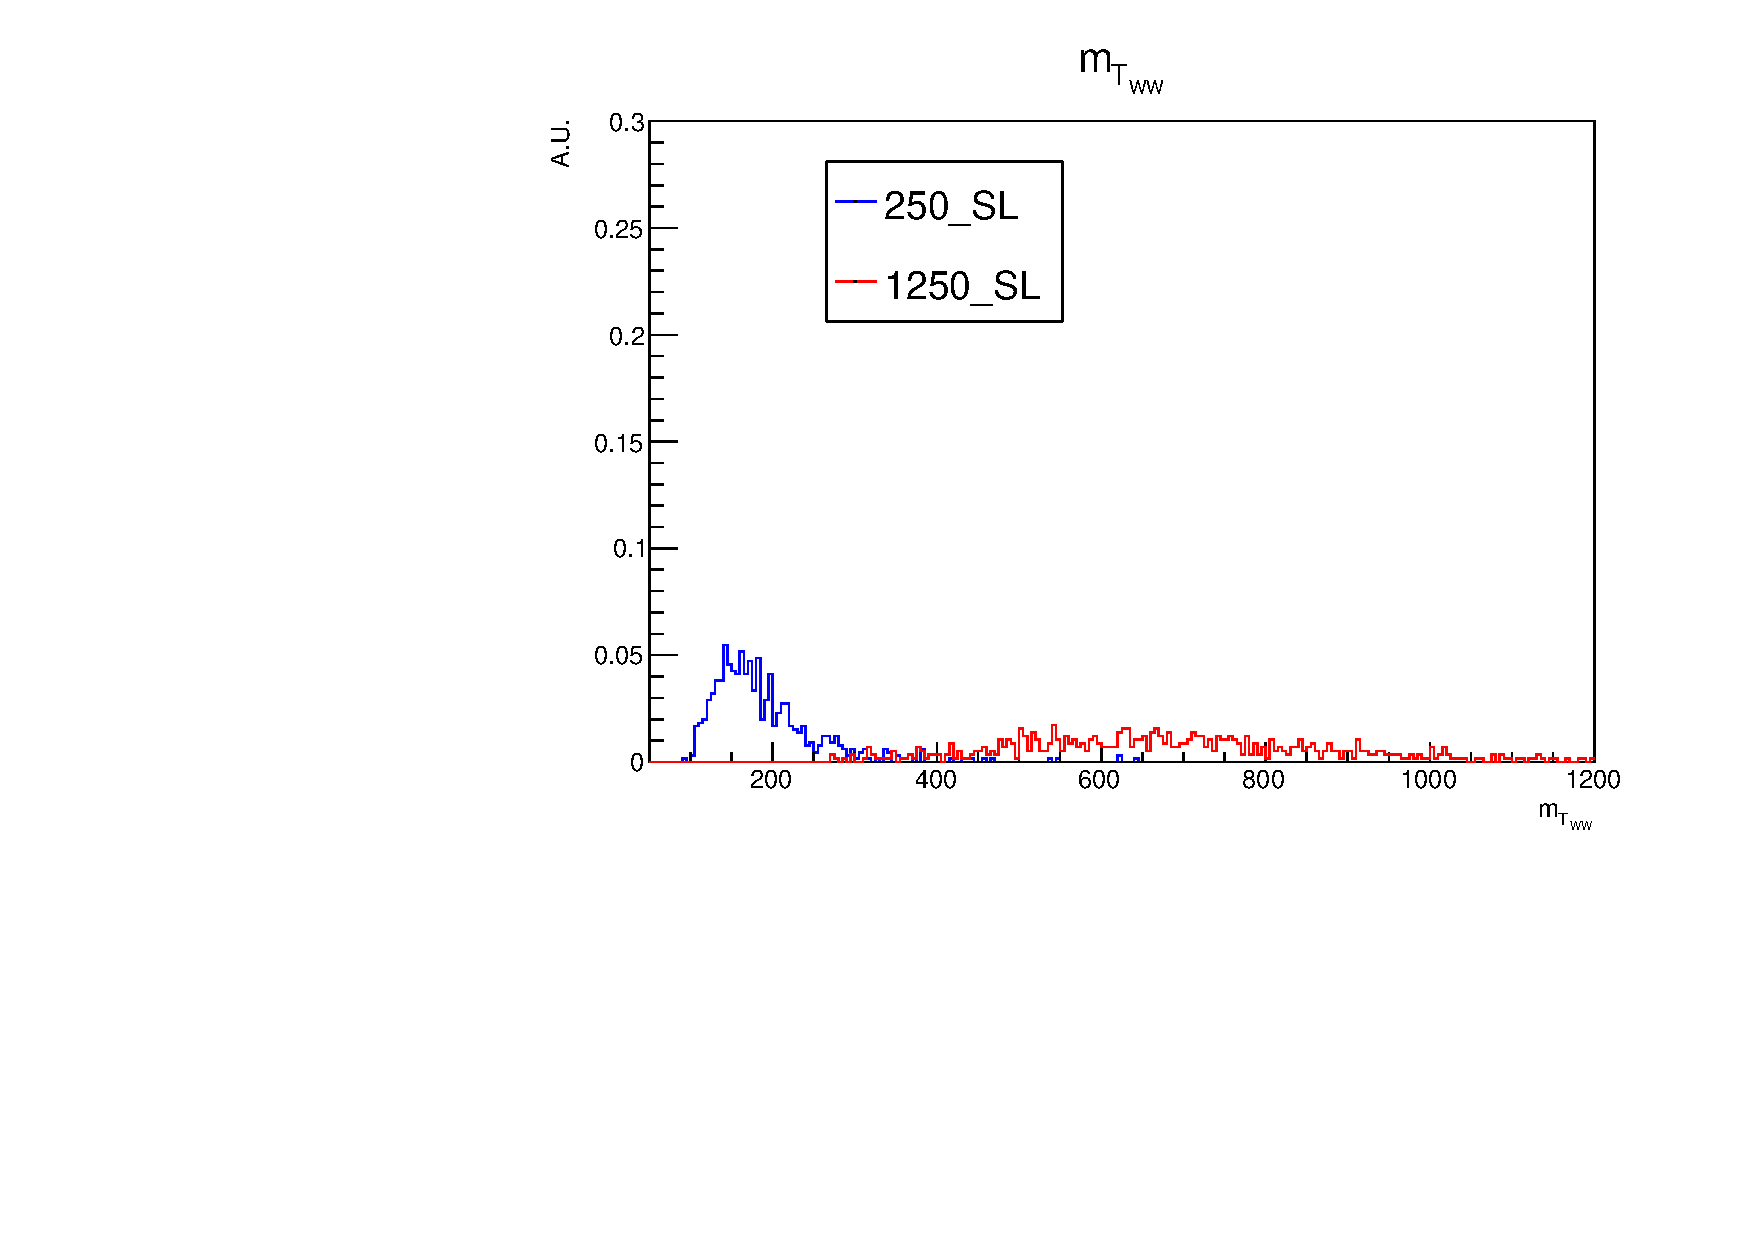
\includegraphics[width=.5\linewidth]{Images/SL_transverse_WWmass.pdf}
% %     \caption{Transverse mass of the di-W pair as reconstructed from the leading lepton, MET and leading/subleading jets.}
% % \end{figure}

% Here it can be seen that the invariant mass of the diphoton object peaks around the SM Higgs mass of $\approx 125 GeV$ for all three decay modes and both mass points. It should be noted however that the distributions are not as well peaked in the fully hadronic case, possibly because there may be jets which are faking photons. It can also be seen that the $p_{T}$ distribution of the Higgs decaying into two photons shifts to the right in the case of the 1250 GeV radion, for all three decay modes, because the Higgs bosons are more likely to be boosted. Finally, when looking at the semi-leptonic channel in figure 12, the invariant mass of two jets which are matched with GEN quarks is seen to have a peak around 80 GeV corresponding to the on-shell W boson, and a peak at a lower mass corresponding to the off-shell W boson. 
% When running on 2016, 2017 and 2018 data, the data samples planned to be used are the DoubleEG data sets, containing events that should have two electrons, two photons, or an electron and a photon object. The HLT paths applied to events in this primary data set for 
% \begin{figure}[H]
% \centering
% \begin{BVerbatim}
% HLT_Diphoton30_18_R9Id_OR_IsoCaloId_AND_HE_R9Id_Mass90
% \end{BVerbatim}
% \end{figure}
% for 2016 data, and 
% \begin{figure}[H]
% \centering
% \begin{BVerbatim}
% HLT_Diphoton30_22_R9Id_OR_IsoCaloId_AND_HE_R9Id_Mass90
% \end{BVerbatim}
% \end{figure}
% for 2017 data. These will be selected because they are expected to contain $H\rightarrow \gamma\gamma$ events, which could contain $HH\rightarrow WW\gamma\gamma$ events.